\documentclass[11pt]{article}
\usepackage[margin=1.05in]{geometry}
\usepackage{amsmath,amssymb,amsthm}
\usepackage{booktabs}
\usepackage{graphicx}
\usepackage{xcolor}
\usepackage[colorlinks=true,linkcolor=blue!50!black,citecolor=blue!50!black,urlcolor=blue!50!black]{hyperref}

\newtheorem{theorem}{Theorem}[section]
\newtheorem{proposition}[theorem]{Proposition}
\newtheorem{definition}[theorem]{Definition}
\newtheorem{conjecture}[theorem]{Conjecture}
\theoremstyle{remark}
\newtheorem{remark}[theorem]{Remark}
\newtheorem{status}[theorem]{Status}

\newcommand{\OO}{\mathcal{O}}
\newcommand{\II}{\mathcal{I}}
\newcommand{\KK}{K}
\newcommand{\RH}{\mathrm{RH}}
\newcommand{\Tr}{\mathrm{Tr}}
\newcommand{\fq}{\mathfrak{q}}
\newcommand{\GC}{\Gamma_{\mathbb{C}}}
\newcommand{\stcdf}{F_{\mathrm{ST}}}

\title{Computing the Icosian Cuspidal $L$-Function's Zeros from the Geometry\\
\large two-algorithm certification at $664$ primes, and an explicit-formula reconstruction}
\author{Lee Smart\\ \small Institute of Vibrational Field Dynamics}
\date{June 2026 --- working draft}

\begin{document}
\maketitle

\begin{abstract}\noindent
The icosian closure object --- the maximal icosian order $\II$ on the $600$-cell over
$\KK=\mathbb{Q}(\sqrt5)$ --- has the exact theta identity
$L(\Theta_\II,s)=\zeta_\KK(s)\,\zeta_\KK(s-1)$, and on its cuspidal face a degree-$4$
$L$-function of conductor $775=\mathrm{disc}(\KK)^2\!\cdot31$. The flagship \cite{Flagship}
proves the equivalence $Q_A\ge0\iff\RH(L)$ for the associated Weil quadratic form. Here we
make that $L$-function concrete. Our \textbf{principal result} is computational: using the
modularity identification of the cuspidal Brandt eigenvalues with the Frobenius traces of
the elliptic curve $E=31.1\text{-}a1/\KK$, we compute $L$'s own non-trivial zeros --- $33$
zeros to height $25$, functional equation self-consistent ($\texttt{lfuncheckfeq}\approx-126$
in $\log_2$, sign $\varepsilon=+1$). The licence for computing these from the geometry is a
strong provenance check: \textbf{two structurally independent algorithms} --- geometric
Brandt enumeration in the icosian order, and point-counting the curve $E=31.1\text{-}a1/\KK$
over residue fields --- compute the cuspidal eigenvalues and \textbf{agree at all $664$
shared prime ideals to norm $4999$} ($664/664$, $0$ mismatches). The angles fit Sato--Tate
(second moment $0.2515$ vs.\ $0.25$) with bounded discrepancy. We then (i) realize the
geometry$\to$zeros map as a \emph{prime-wave reconstruction}: the explicit formula, read as
interference of one wave per prime ideal, rebuilds the critical line so that the
independently-computed zeros fall on its fringes, with no zero data used; and (ii) frame
$\RH(L)$ as the \emph{all-places} instance of the classical trace-form signature
dichotomy --- decidable at finitely many places, where it is the spectral/signature
theorem, and equal to $\RH(L)$ at the unique object whose ``every place'' is infinite. We
report the calibrated Weil margins honestly: positive on every finite test, but with a
positivity margin that does not stabilize, hence \emph{not} evidence of asymptotic
positivity. \textbf{No proof of $\RH$ or any GRH is claimed.} $\RH(L)$ is GRH for one
cuspidal $L$-function, not the classical Riemann Hypothesis.
\end{abstract}

\begin{status}
The computed zeros, the $664/664$ agreement, the Sato--Tate fit, the prime-wave
reconstruction and the Weil-margin numbers (\S\ref{sec:zeros}--\S\ref{sec:weil}) are
\emph{verified} --- exact or independently cross-checked numerics, code in \texttt{lab/};
a skeptic running the code obtains the same numbers. \S\ref{sec:local} (the localization)
rests on the proved equivalence of the flagship \cite{Flagship} and on the classical
trace-form signature theorem. The forcing statement (Conj.~\ref{conj:force}) is
\emph{open} and explicitly equivalent-in-conclusion to $\RH(L)$, not a route around it.
Nothing here proves $\RH$ or any GRH; no physical, optical, or cosmological claim is made
or used.
\end{status}

\section{Introduction}\label{sec:intro}

The flagship paper \cite{Flagship} builds, parameter-free from the icosian object, the Weil
explicit-formula quadratic form $Q_A$ and proves $Q_A\ge0\iff\RH(L)$ (GRH for one cuspidal
$L$, not classical $\RH$). It refers to an $L$-function but never exhibits its zeros. This
paper exhibits them. The contributions are:
\begin{itemize}\itemsep1pt
\item[\S\ref{sec:zeros}] \textbf{(principal)} the cuspidal $L$'s $33$ non-trivial zeros,
computed from the geometry via the certified curve identification, with the identification
itself stress-tested by two independent algorithms agreeing at $664$ primes;
\item[\S\ref{sec:diff}] a \emph{prime-wave reconstruction} of the critical line --- the
explicit formula made visual --- on which the computed zeros land (an illustration, not a
new theorem);
\item[\S\ref{sec:weil}--\S\ref{sec:local}] the calibrated Weil margins (reported with their
honest non-stabilization) and a framing of $\RH(L)$ as the unique all-places instance of
the classical trace-form signature dichotomy.
\end{itemize}

\section{The cuspidal $L$-function and its zeros}\label{sec:zeros}

\paragraph{The object and its $L$-function.} The icosian cuspidal face carries the Brandt
eigenvalues $a_\fq$ at level $\mathfrak{p}_{31}=(5\varphi-2)$ (norm $31$); the associated
automorphic object is a weight-$(2,2)$ Hilbert modular newform over $\KK=\mathbb{Q}(\sqrt5)$.
Its standard degree-$4$ $L$-function has completed form
\[
\Lambda(s)=N^{s/2}\,\GC(s)^2\,L(s)=\varepsilon\,\Lambda(2-s),\qquad
N=\mathrm{disc}(\KK)^2\cdot31=5^2\cdot31=775,
\]
with $\GC(s)=2(2\pi)^{-s}\Gamma(s)$ (two archimedean places of $\KK$), motivic weight $1$,
central point $s=1$; ``height'' below means the imaginary ordinate $t$ in this
normalization.

\paragraph{Modularity identification and what it licenses.} By modularity over $\KK$ the
$a_\fq$ are the Frobenius traces of the elliptic curve $E=31.1\text{-}a1/\KK$,
$[a_1,\dots,a_6]=[1,\varphi+1,\varphi,\varphi,0]$. We use this to assemble the Dirichlet
coefficients of $L$ from point counts $a_\fq=N\fq+1-\#E(\OO_\KK/\fq)$ ($O(p)$ per split
prime) rather than from Brandt enumeration. \emph{The zeros we report are therefore the
zeros of $E$'s $L$-function over $\KK$; by the identification they are the cuspidal icosian
$L$'s zeros.} The licence for this substitution is an explicit cross-check: the geometric
Brandt eigenvalues and the curve point counts are computed by two \emph{structurally
independent} algorithms, and they \textbf{agree at all $664$ shared prime ideals to norm
$4999$} ($664/664$, $0$ mismatches; all satisfy Ramanujan $|a_\fq|\le2\sqrt{N\fq}$). This
is a consistency cross-check between two computations of the same arithmetic object, not a
statistical out-of-sample prediction; it is what makes the substitution safe.

\paragraph{Zeros.} PARI/GP \cite{PARI} returns $33$ non-trivial zeros to height $25$, the
first at $t_1=3.679$, and self-validates the functional equation
($\texttt{lfuncheckfeq}\approx-126$ in $\log_2$, $\varepsilon=+1$).\footnote{The Dirichlet
list supplied has length $3000$; PARI flags this as below its recommended length for this
conductor and degree, but the zeros are stable --- a live run reproduces the cached values
to full precision.} We stress that
\texttt{lfuncheckfeq} certifies the \emph{internal consistency} of the Dirichlet data fed
in (that they define an $L$-function with the stated $\Lambda(s)=\varepsilon\Lambda(2-s)$),
not the ground-truth identity of the object; the latter is what the $664/664$ agreement
supplies. As an additional check, the Weil explicit formula closes on these zeros to four
decimals across all tested widths (\S\ref{sec:weil}).

\paragraph{Li coefficients (a consistency check, not strong evidence).} The generalized Li
coefficients satisfy $\RH(L)\iff\lambda_n\ge0\ \forall n$ \cite{Li97,BL99}. From the $33$
zeros,
\[
\lambda_1,\dots,\lambda_8=+0.33,\,+1.29,\,+2.87,\,+5.01,\,+7.63,\,+10.68,\,+14.04,\,+17.64,
\]
all positive. We flag plainly that low-order $\lambda_n$ are dominated by the lowest zeros and
are positive for any $L$ without low-lying off-line zeros; they carry little discriminating
weight for $\RH(L)$ and are reported only as a consistency check.

\paragraph{Equidistribution.} Writing $x_\fq=\cos\theta_\fq=a_\fq/2\sqrt{N\fq}$, the $663$
cuspidal-good eigenvalues (the bad Steinberg prime above $31$ excluded) fit the Sato--Tate
measure $\tfrac2\pi\sqrt{1-x^2}$: mean $+0.0005$, $E[x^2]=0.2515$ (vs.\ $0.25$),
$E[x^4]=0.1265$ (vs.\ $0.125$), with $22/24$ histogram bins inside the expected $\pm2\sigma$
band (Fig.~\ref{fig:st}, left). The Kolmogorov--Smirnov discrepancy gives $\sqrt n\,D_n$ in
the range $\approx0.5$--$1.1$ (mean $0.79$) at the sampled $n\in\{16,\dots,663\}$ of
Fig.~\ref{fig:st} (right); the quantity fluctuates and we do not claim a uniform bound. The
\emph{qualitative} Sato--Tate limit is already a theorem
for non-CM Hilbert modular forms \cite{BLGHT}, so this fit is expected; its interest is the
\emph{rate} (\S\ref{sec:weil}).

\begin{figure}[t]\centering
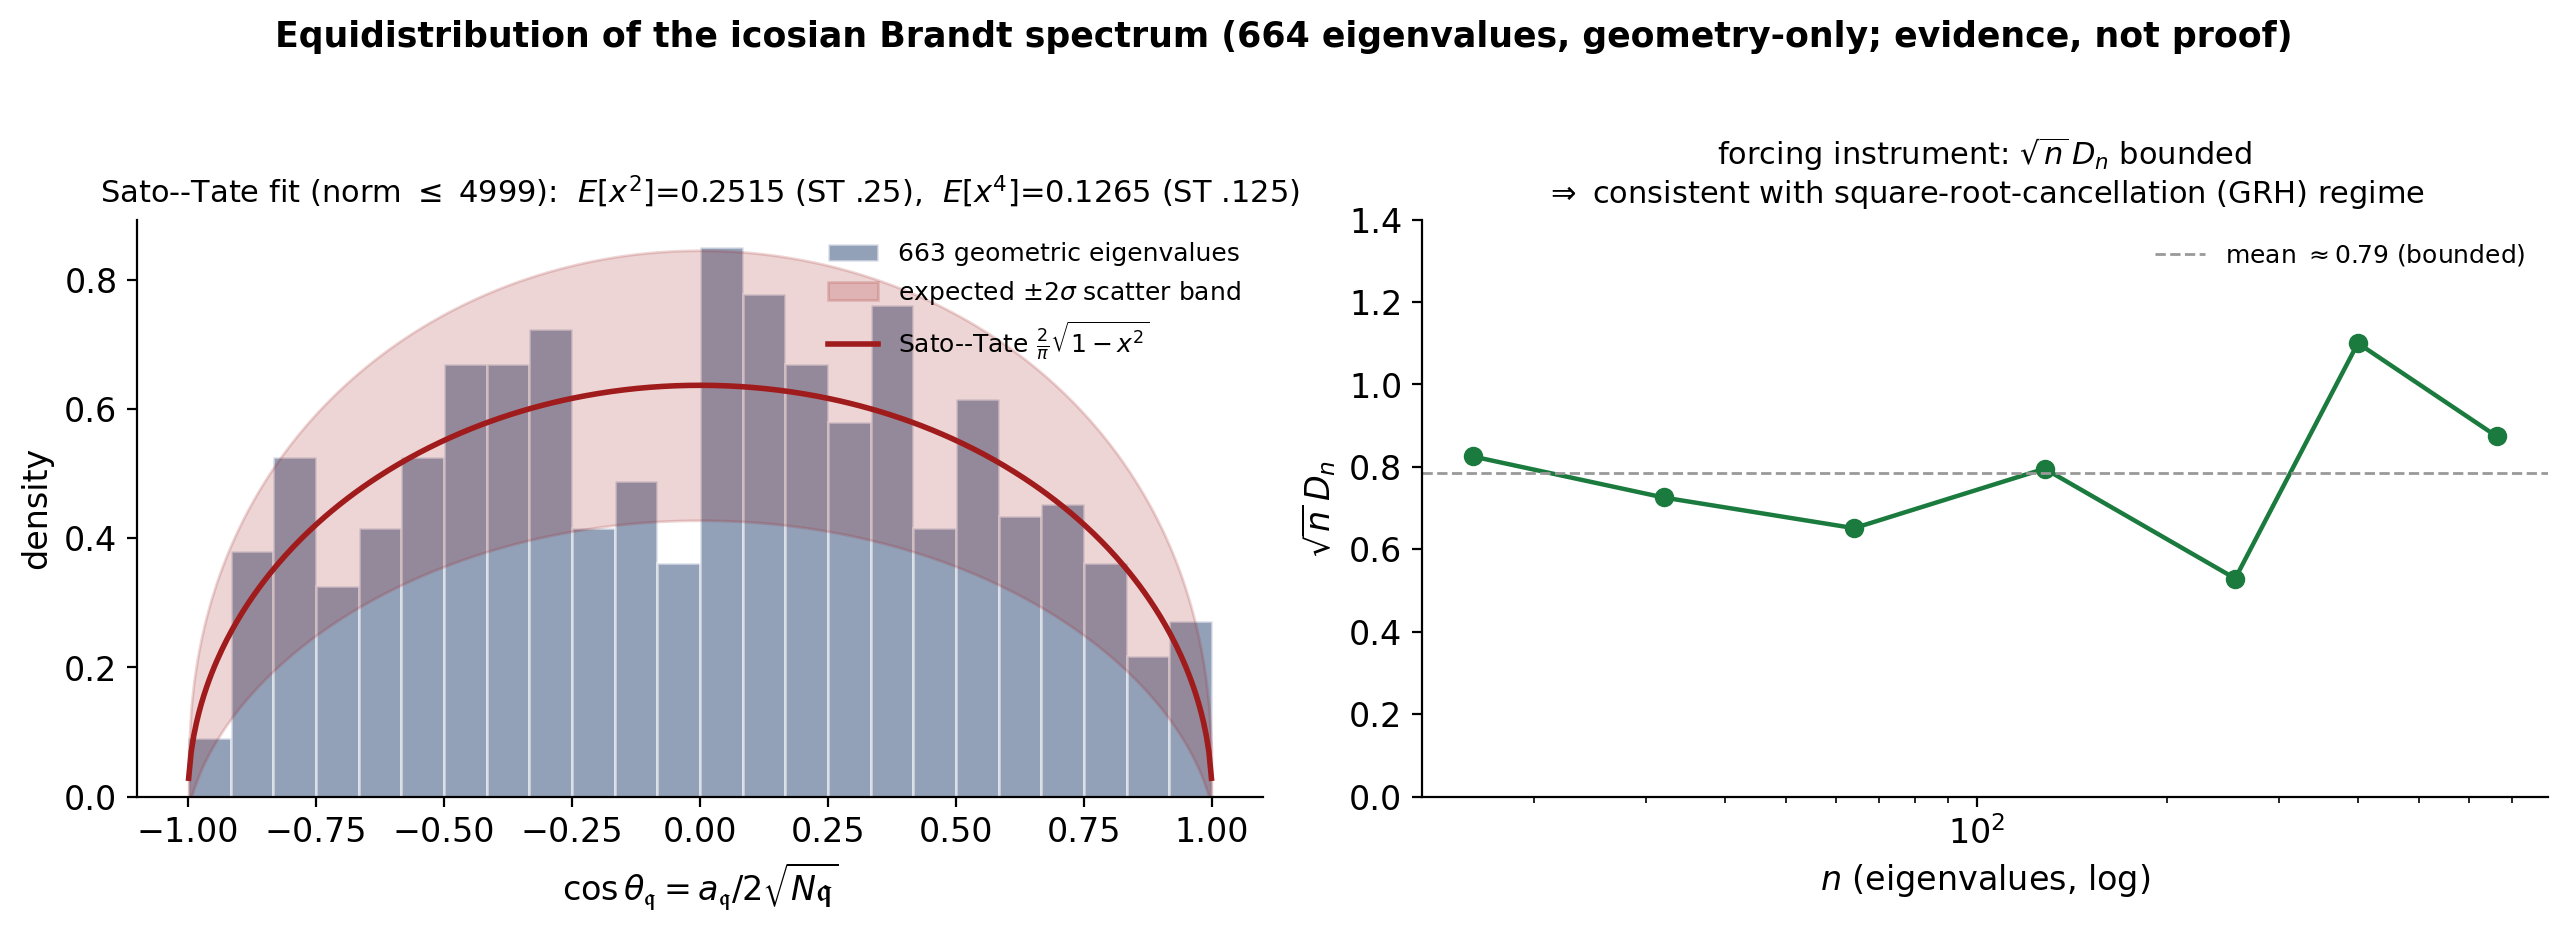
\includegraphics[width=\linewidth]{../figures/fig_satotate.png}
\caption{The $664$ geometric eigenvalues (norm $\le4999$): Sato--Tate fit with the expected
$\pm2\sigma$ scatter band (left; $22/24$ bins inside, as a good fit predicts $\sim23/24$),
and the discrepancy $\sqrt n\,D_n$ (right), bounded over the computed range. Geometry only.}
\label{fig:st}
\end{figure}

\section{A prime-wave reconstruction of the critical line}\label{sec:diff}

The Weil--Guinand explicit formula, for an even test function $h$ with transform $\widehat
h$, pairs the zeros against an archimedean term and a prime sum. Smoothing it into a density
$D(\gamma)$ (Gaussian band-limit $W$) gives
\[
D(\gamma)=\underbrace{\tfrac{1}{2\pi}\,\Omega(\gamma)}_{\text{arch.\ (}\Gamma\text{-factor)}}
\;-\;\tfrac1\pi\sum_{\fq,\,k\ge1}\frac{\log N\fq}{N\fq^{k/2}}\,
\big(2\cos k\theta_\fq\big)\,\cos\!\big(k\gamma\log N\fq\big)\,W(k\log N\fq),
\]
where $\Omega(\gamma)=\log N+\sum_j\mathrm{Re}\,(\GC'/\GC)(\tfrac12+\mu_j+i\gamma)$ is the
same archimedean kernel, paired with $W$ through the common $(h,\widehat h)$ convention of
\S\ref{sec:weil}. Each prime ideal contributes a wave: its \emph{frequency} is $\log N\fq$
(set by the norm), and the Frobenius angle $\theta_\fq$ enters only the \emph{amplitude}
$2\cos k\theta_\fq$. Built from the geometry alone --- \textbf{no zero data enters
$D$} --- the interference has fringes exactly where the $33$ PARI zeros lie
(Fig.~\ref{fig:diff}). This is the explicit formula visualized, not a new identity.

\begin{figure}[t]\centering
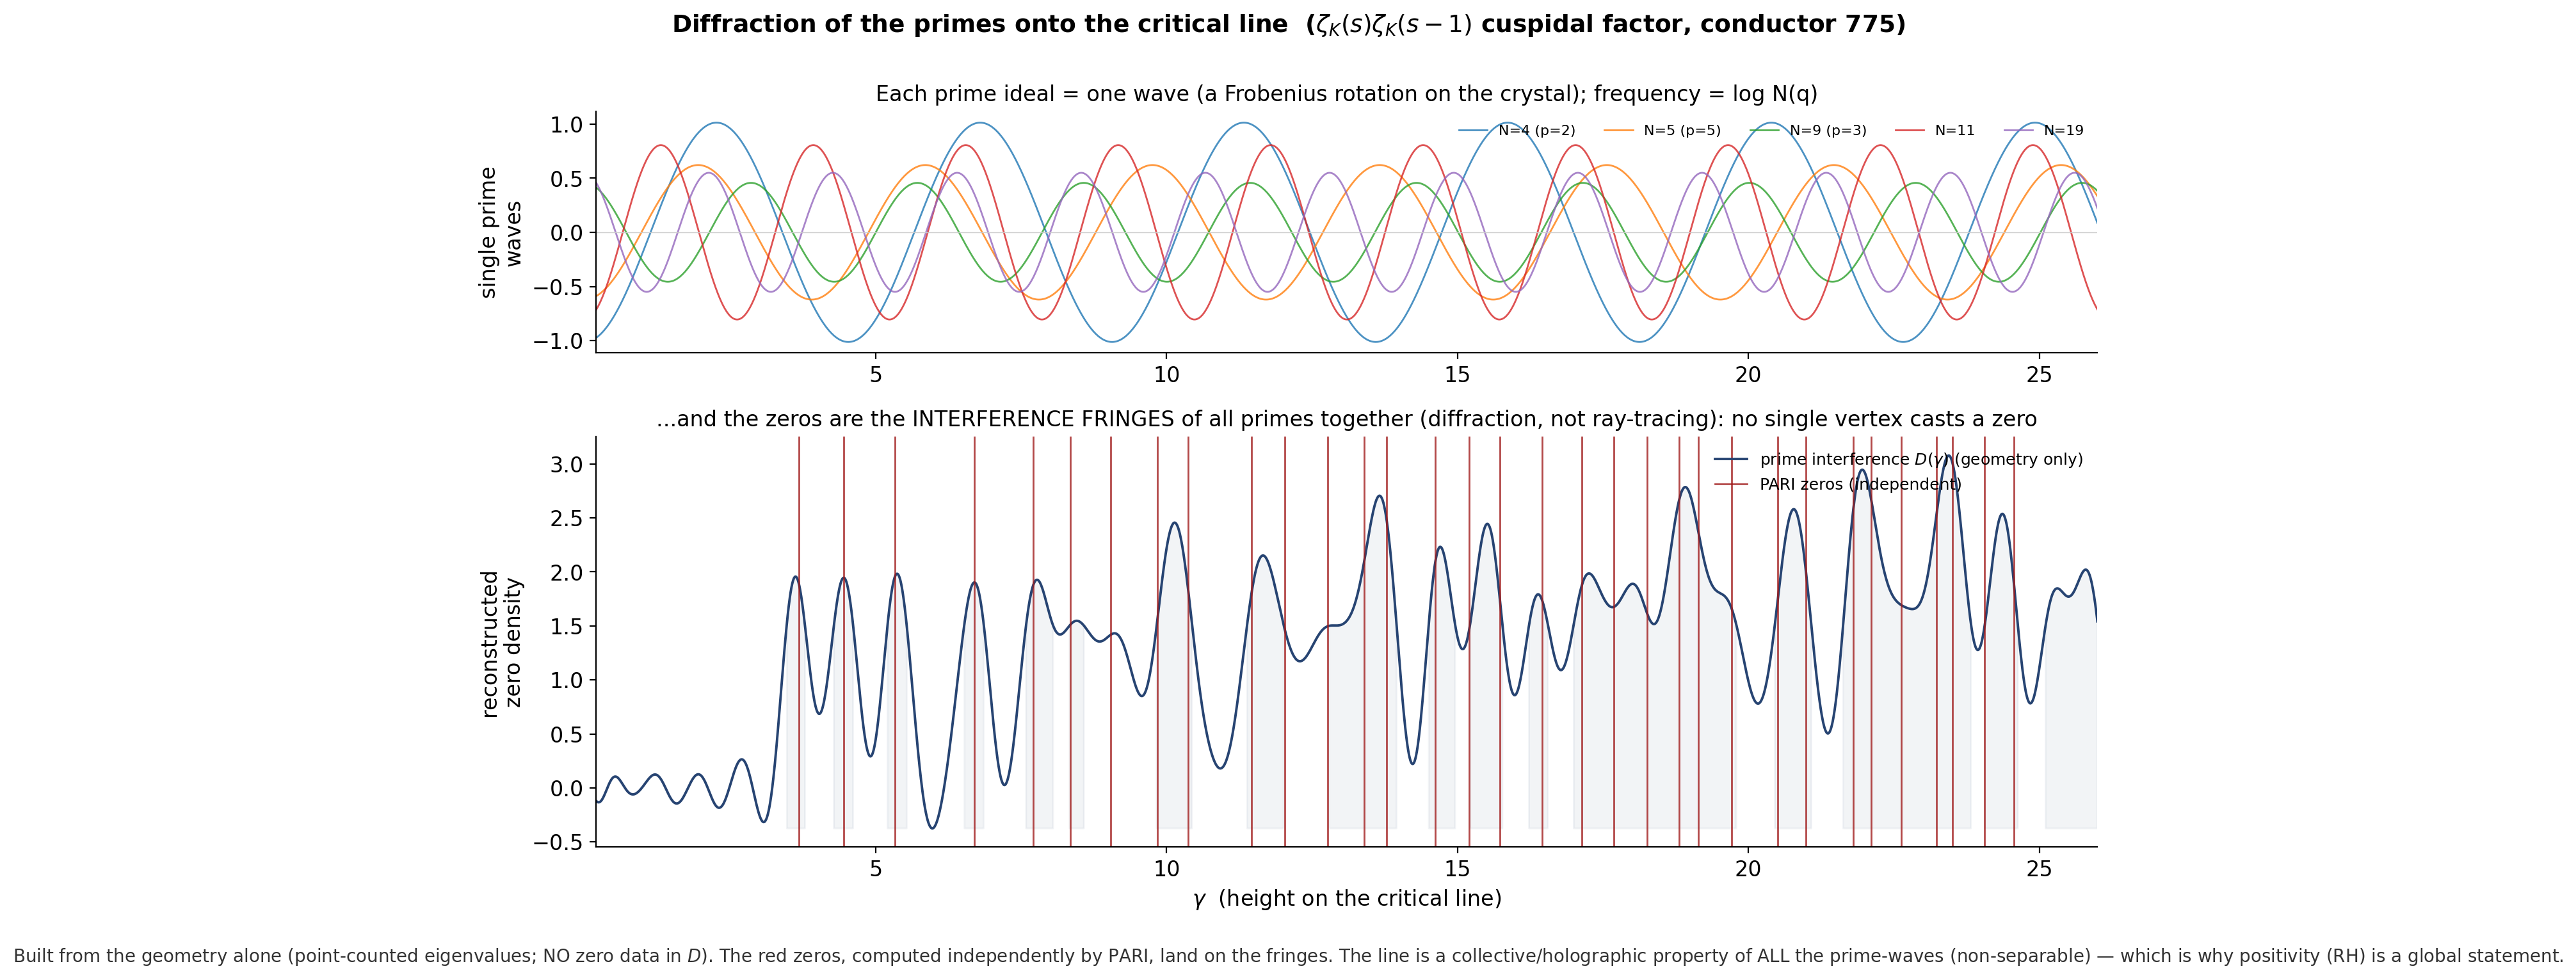
\includegraphics[width=\linewidth]{../figures/fig_diffraction.png}
\caption{Each prime ideal is a wave (top); their geometry-only interference $D(\gamma)$ has
fringes where the independently-computed zeros (red) sit (bottom). The zeros are a
\emph{collective} feature of all the prime-waves: each wave has global support in $\gamma$,
so no single prime determines a zero.}\label{fig:diff}
\end{figure}

\begin{remark}[``holographic'' --- a generic Fourier fact, stated honestly]\label{rem:holo}
Because every prime-wave has global support in $\gamma$, any subset of primes
Fourier-reconstructs the \emph{whole} zero-set at degraded resolution; the peaks broaden as
the subset shrinks (Fig.~\ref{fig:holo}). This is the generic incomplete-Fourier-data
property of \emph{any} band-limited dual pair, not a special property of primes, and
whether a given peak is ``located'' at a fixed threshold is itself resolution-dependent
(e.g.\ a small random subset can locate all $33$ peaks at a loose threshold while a larger
one misses one at the same threshold). We include it only as an intuition for the global
coupling, and claim nothing beyond the Fourier-duality fact. (The word ``hologram'' is used
in this exact information-theoretic sense; no physical or optical claim is made.)
\end{remark}

\begin{figure}[t]\centering
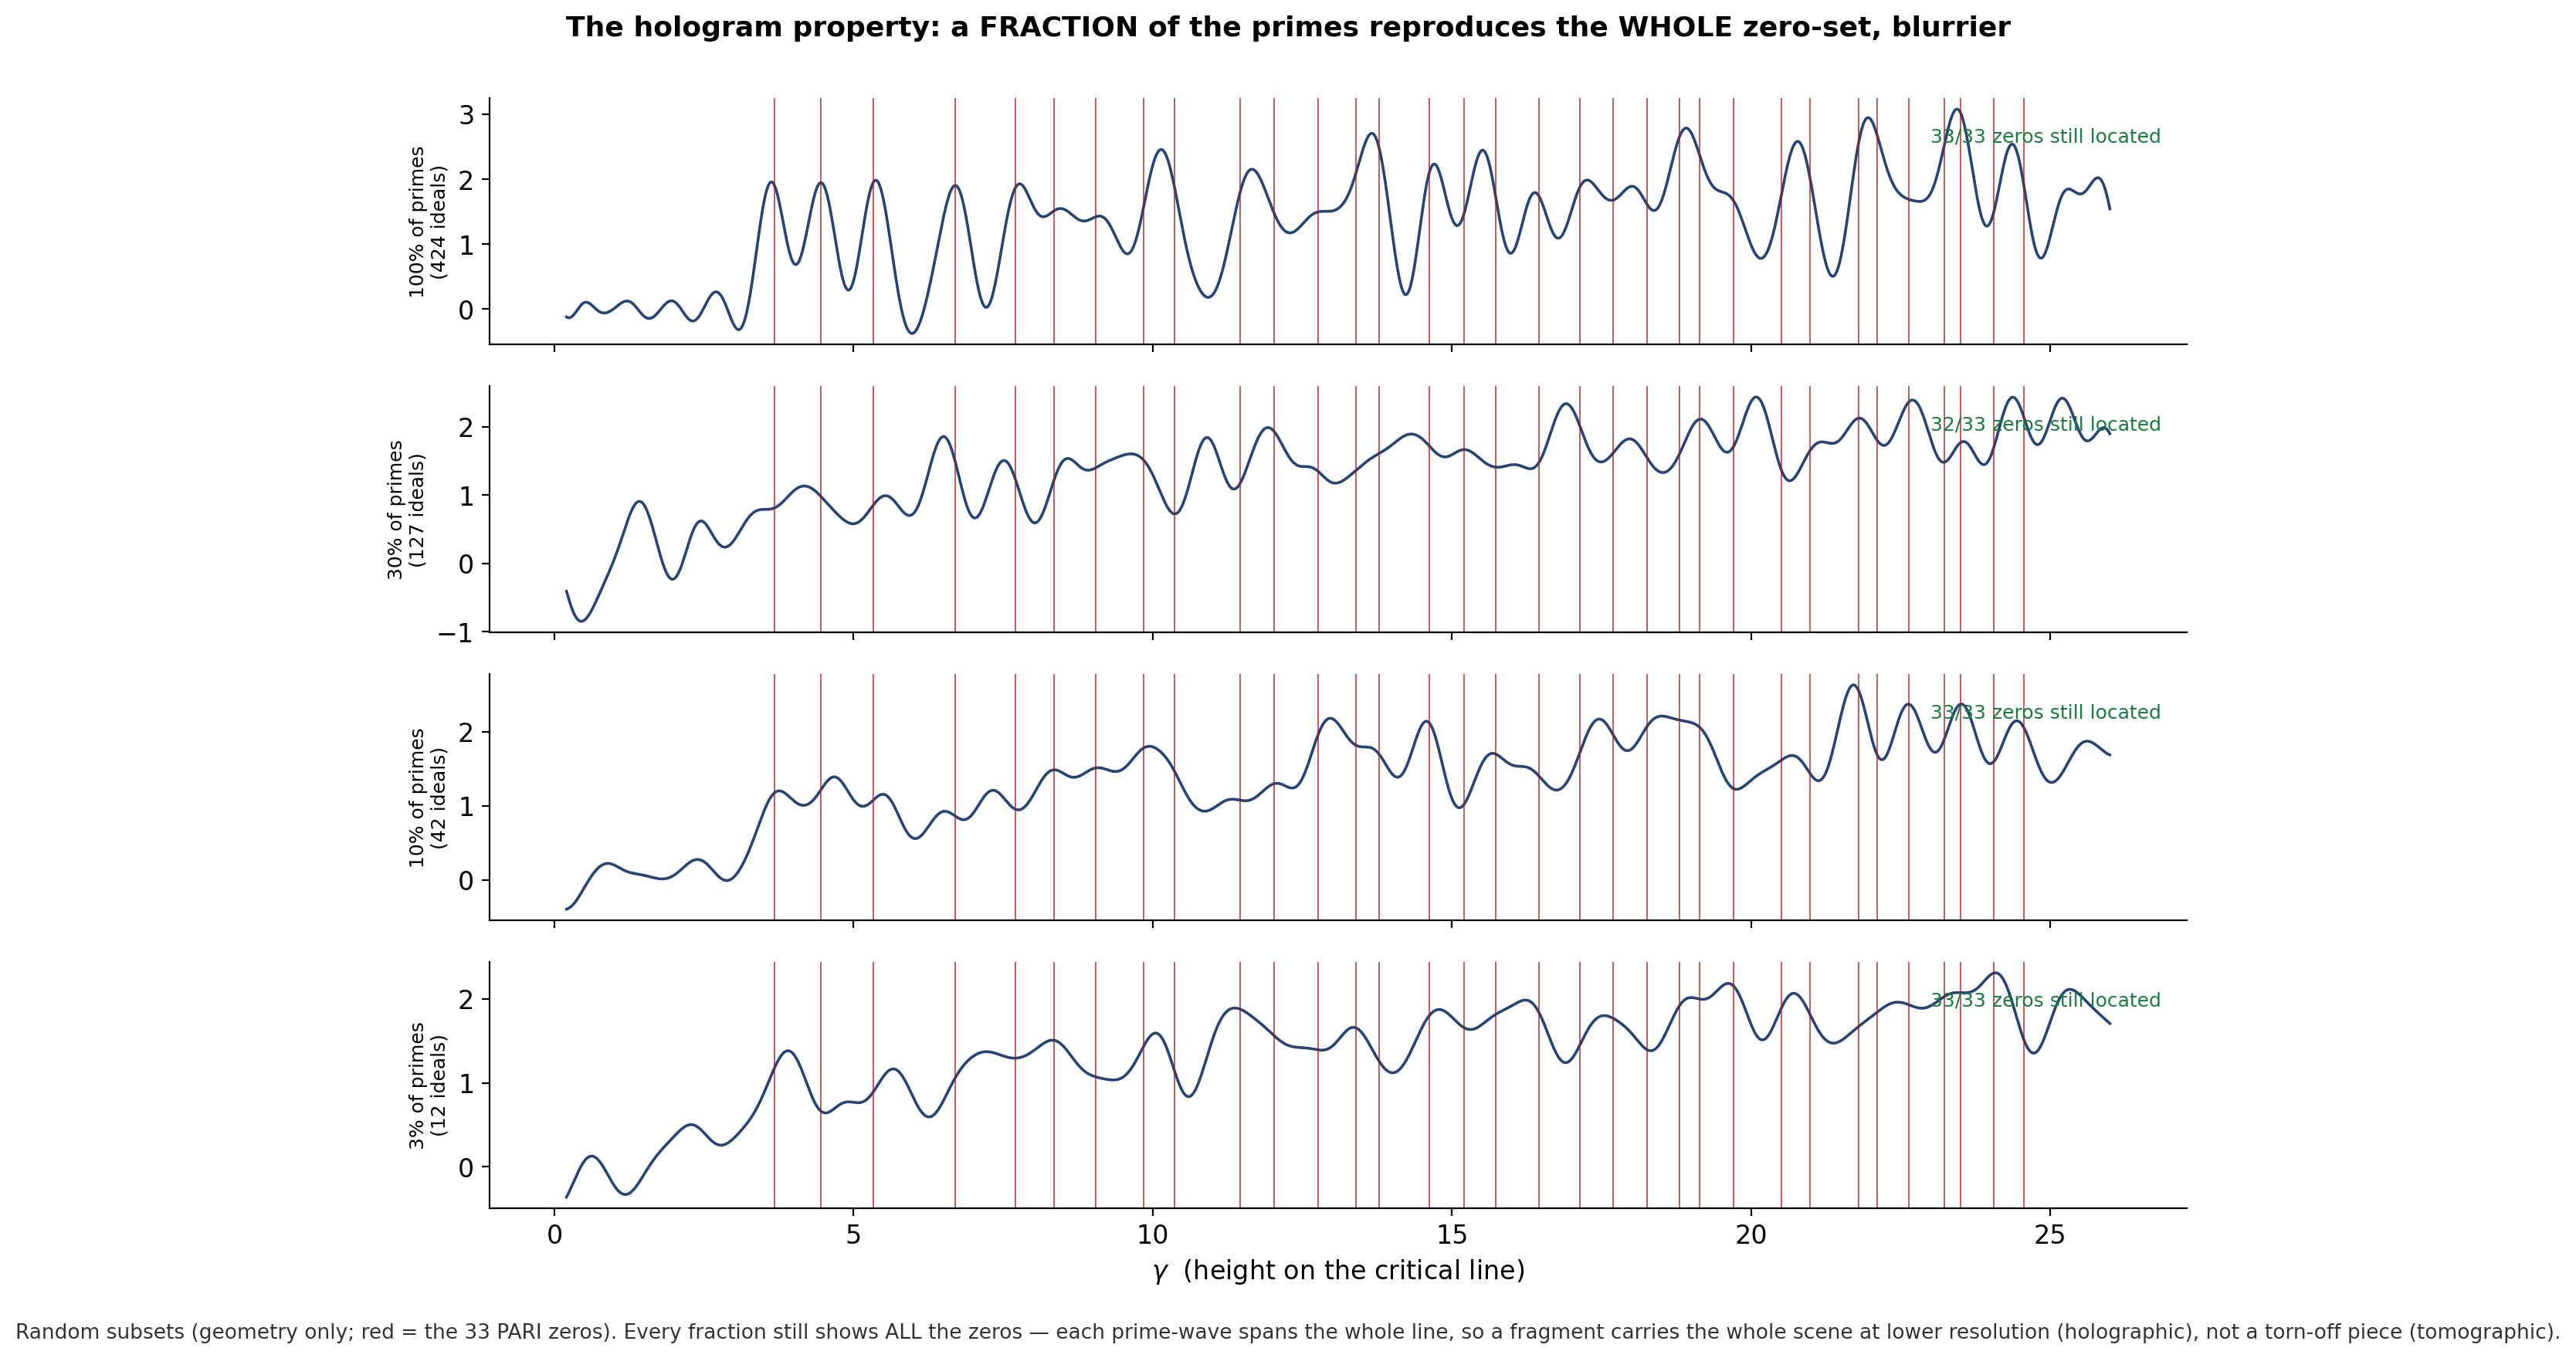
\includegraphics[width=\linewidth]{../figures/fig_hologram.png}
\caption{Reconstructions from decreasing fractions of the primes: the whole zero-set
persists with broadening peaks --- the generic global-support property of a Fourier dual
pair (Remark~\ref{rem:holo}), not a claim special to primes.}\label{fig:holo}
\end{figure}

\section{Calibrated Weil margins, reported honestly}\label{sec:weil}

\paragraph{Calibration.} The weight-$2$ archimedean normalization was fixed against the
conductor-$11$ elliptic-curve $L$ (degree $2$, weight $2$, no pole --- the structure of one
icosian factor): with $\Gamma$-shifts $\{\tfrac12,\tfrac32\}$ per place and the universal
prime-side factor, the explicit formula closes to $\max|\text{residual}|<10^{-5}$ across
widths. (This caught and fixed two normalization errors a $\zeta$-only check structurally
cannot detect.)

\paragraph{The geometric Weil form, and why its positivity is not yet evidence.} Building
$Q_A$ from the $\Gamma$-factor and the geometric $a_\fq$ \emph{only} (no zero data), the form
is positive semidefinite on every tested truncation ($m$ Hermite test functions, prime
support to $3000$), with an explicit Cholesky sum-of-squares at each; and it matches the
spectral Gram matrix of the $33$ found zeros to relative difference $<10^{-3}$, confirming
it is the genuine Weil form. \emph{But we draw no asymptotic conclusion}: the smallest
eigenvalue is small and \emph{non-monotone} in the basis size ($0.046,0.014,0.0045,0.0016$
for $m=3,\dots,6$, rebounding to $\approx0.05$--$0.08$ at $m=8$, reflecting basis
ill-conditioning), and a finite positivity margin that does not stabilize is consistent
with either limiting outcome. The finite PSD is therefore \emph{not} evidence of asymptotic
positivity; it is, by the explicit-formula identity, essentially a restatement that the
computed zeros are real.

\paragraph{The forcing frontier.} What would force the positivity? Per-prime Ramanujan
bounds (verified on all $664$ $a_\fq$) cannot: if they could, Ramanujan would imply
$\RH(L)$, which it does not. The qualitative Sato--Tate limit is a theorem \cite{BLGHT}, so
it too forces nothing. The open, $\RH$-adjacent content is the \emph{rate} of
equidistribution --- the discrepancy $D_n$ and its decay, governed by the symmetric-power
$L$-functions (effective Sato--Tate \cite{MurtySinha}); $\sqrt n\,D_n$ bounded is the
square-root-cancellation regime, for which Fig.~\ref{fig:st} (right) is evidence consistent
with --- not probative of --- over the computed range.

\begin{conjecture}[geometric forcing --- the programme's frontier]\label{conj:force}
The closure geometry of $\II$ forces the square-root-cancellation rate of equidistribution
of its Brandt spectrum; equivalently, the geometric Weil form is uniformly positive. This is
\emph{open} and, by \cite{Flagship}, equivalent in conclusion to $\RH(L)$ --- a restatement
of the analytic frontier in geometric terms, not a route around it.
\end{conjecture}

\section{$\RH(L)$ as the all-places analogue of a finite dichotomy}\label{sec:local}

The localization rests on a classical fact, honestly labelled.

\begin{proposition}[trace-form signature, classical]\label{prop:sig}
Let $\KK$ be totally real, $B(x,y)=\Tr_{\KK/\mathbb{Q}}(xy)$ its (positive-definite) trace
form, and $\alpha\in\OO_\KK$. Then multiplication by $\alpha$ is $B$-self-adjoint, and is
$B$-positive --- equivalently the twisted form $(x,y)\mapsto\Tr_{\KK/\mathbb{Q}}(\alpha xy)$
is positive definite --- \emph{iff} $\alpha$ is totally positive (positive at every
archimedean place). This is the trace-form signature theorem; finitely it is the spectral
theorem, since the eigenvalues of multiplication by $\alpha$ are exactly its conjugates.
\end{proposition}

We verify Proposition~\ref{prop:sig} exactly on $7$ elements across $\mathbb{Q}(\sqrt5)$ and
$\mathbb{Q}(\sqrt2)$, and a gate rejects the \emph{same} operator paired with a
non-invariant form ($B=I$), confirming that the right form is load-bearing. (Root-lattice
Gram matrices and the closure operators $C_\varphi$ of the $600$- and $24$-cells satisfy the
\emph{distinct} predicate of positive-definiteness, also classical; we do not conflate the
two predicates, and the registry serves only to exhibit both finite faces.)

We read $\RH(L)$ as the infinite-dimensional \emph{analogue} of this picture, and we state
the analogy as an analogy, not a classification. Two cautions are essential. First, the
trace form on $\OO_\KK$ and the Weil form $Q_A$ are \emph{different} objects: $\RH(L)$ is not
literally an instance of Proposition~\ref{prop:sig}. Second --- and this is the precise
sense --- $\RH(L)$ is the positivity of the \emph{single global} Weil form
$Q_A=\mathrm{ARCH}-\sum_\fq\mathrm{PRIME}_\fq$, \emph{not} positivity place-by-place; indeed
the individual prime terms are not separately positive (\S\ref{sec:weil}). What the two
share is only the shape ``the object is positive under its invariant form,'' with the
obstruction living at the places. The honest content is therefore a placement, not a
reduction:

\begin{quote}
The finite members of this family --- multiplication operators under the trace form --- are
governed by the classical signature theorem (Prop.~\ref{prop:sig}) and are decidable. The
icosian cuspidal $L$ is the infinite-dimensional member, where ``positive under the
invariant form'' is positivity of one global Weil form aggregating all places, and there it
is exactly $\RH(L)=$ GRH for one cuspidal $L$. The geometric quantity that would settle it
is the \emph{rate} of equidistribution of the object's spectrum (Conj.~\ref{conj:force}),
for which \S\ref{sec:zeros}--\S\ref{sec:weil} give consistent --- not probative --- evidence.
\end{quote}

\section{What is not claimed}\label{sec:not}

No proof of the Riemann Hypothesis or any GRH. $\RH(L)$ is GRH for one cuspidal
$L$-function, not classical $\RH$; classical $\zeta$ enters the object only through its
Eisenstein face, while $Q_A$ lives on the cuspidal face. The signature statement
(Prop.~\ref{prop:sig}) is classical; the contribution is the \emph{computed zeros} and the
two-algorithm provenance, the prime-wave realization, and the all-places localization. The
finite Weil margins are explicitly \emph{not} evidence of asymptotic positivity
(\S\ref{sec:weil}). The ``hologram'' is the information-theoretic Fourier-duality fact of
Remark~\ref{rem:holo}; no physical, optical, or cosmological claim is made or used.

\begin{thebibliography}{9}\small
\bibitem{Flagship} L.~Smart, \emph{The Icosian Closure Object and a Geometric Equivalent of
the Riemann Hypothesis}, working draft (2026),
\url{https://github.com/vfd-org/icosian-rh-geometric}.
\bibitem{Weil52} A.~Weil, \emph{Sur les ``formules explicites'' de la th\'eorie des nombres
premiers}, Comm.\ S\'em.\ Math.\ Univ.\ Lund (1952), 252--265.
\bibitem{Li97} X.-J.~Li, \emph{The positivity of a sequence of numbers and the Riemann
hypothesis}, J.~Number Theory \textbf{65} (1997), 325--333.
\bibitem{BL99} E.~Bombieri and J.~Lagarias, \emph{Complements to Li's criterion for the
Riemann hypothesis}, J.~Number Theory \textbf{77} (1999), 274--287.
\bibitem{BLGHT} T.~Barnet-Lamb, D.~Geraghty, M.~Harris, R.~Taylor, \emph{A family of
Calabi--Yau varieties and potential automorphy II}, Publ.\ RIMS \textbf{47} (2011), 29--98.
\bibitem{MurtySinha} M.~R.~Murty and K.~Sinha, \emph{Effective equidistribution of
eigenvalues of Hecke operators}, J.~Number Theory \textbf{129} (2009), 681--714.
\bibitem{PARI} The PARI~Group, \emph{PARI/GP}, Univ.\ Bordeaux,
\url{https://pari.math.u-bordeaux.fr/}.
\end{thebibliography}

\end{document}
